% answers.tex —— 1963 年·全国卷 · 参考答案与详细解析片段
% 由 tools/generate_projects.py 依来源总账自 1963/1963_数学真题_试题.md + 1963/1963_数学真题_解析正文.md + 1963/1963_数学真题_答案要点.md 生成，勿手改（改源 MD 后重跑）


\gkpart{一、小题}

\begin{answer}
\gksolhead{1}{}

\textbf{题目}：

\Needspace{5\baselineskip}
已知 $\tan\theta=\sqrt2$，求

\nopagebreak[4]
\[
\frac{\cos\theta+\sin\theta}{\cos\theta-\sin\theta}
\]

的值。

\Needspace{4\baselineskip}
\textbf{解析}

\Needspace{5\baselineskip}
因 $\tan\theta=\sqrt2$，分子分母同除以 $\cos\theta$，得到

\nopagebreak[4]
\[
\frac{\cos\theta+\sin\theta}{\cos\theta-\sin\theta}
=\frac{1+\tan\theta}{1-\tan\theta}
=\frac{1+\sqrt2}{1-\sqrt2}
\]

\Needspace{5\baselineskip}
分母有理化：

\nopagebreak[4]
\[
\frac{1+\sqrt2}{1-\sqrt2}
=\frac{(1+\sqrt2)^2}{1-2}
=-3-2\sqrt2
\]

\gkanswer{答案：$-3-2\sqrt2$。}

\end{answer}
\begin{answer}
\gksolhead{2}{}

\textbf{题目}：

（1） 求出复数 $1+\sqrt3i$ 的模数和辐角。

（2） 在直角坐标系 $XOY$ 所在的平面内，以 $A$ 点表示复数 $1+\sqrt3i$，把 $OA$ 绕着 $O$ 点按反时针方向旋转 $150^\circ$，设 $A$ 点到达的位置为 $B$，写出 $B$ 点所表示的复数的代数式。

\Needspace{4\baselineskip}
\textbf{解析}

\gksubpart{（1）}

\Needspace{5\baselineskip}
令 $z=1+\sqrt3i$。其模数为

\nopagebreak[4]
\[
|z|=\sqrt{1^2+(\sqrt3)^2}=2
\]

\Needspace{5\baselineskip}
由于实部为正、虚部为正，辐角主值为 $60^\circ$；因此辐角的一般形式为

\nopagebreak[4]
\[
\arg z=60^\circ+360^\circ k\qquad k\in\mathbb Z
\]
\nopagebreak[4]
\begin{center}\begin{tikzpicture}[>=Stealth,scale=0.95]
  \draw[->] (-1.8,0) -- (1.8,0) node[below right] {$x$};
  \draw[->] (0,-1.55) -- (0,1.65) node[above left] {$y$};
  \draw[->,thick] (0,0) -- (0.72,1.25) node[above right] {$A$};
  \draw[->,thick] (0,0) -- (-0.72,-1.25) node[below left] {$B$};
  \node[below left] at (0,0) {$O$};
\end{tikzpicture}
\end{center}
\nopagebreak[4]
\gksubpart{（2）}

\Needspace{5\baselineskip}
将 $OA$ 逆时针旋转 $150^\circ$ 后，模数不变，辐角主值变为

\nopagebreak[4]
\[
60^\circ+150^\circ=210^\circ
\]

\Needspace{5\baselineskip}
所以点 $B$ 表示的复数为

\nopagebreak[4]
\[
2(\cos210^\circ+i\sin210^\circ)=-\sqrt3-i
\]

\gkanswer{答案（1）：模数为 $2$；辐角主值为 $60^\circ$，一般辐角为 $360^\circ k+60^\circ$（$k\in\mathbb Z$）。}

\gkanswer{答案（2）：$-\sqrt3-i$。}

\end{answer}
\begin{answer}
\gksolhead{3}{}

\textbf{题目}：

如图，$AB$ 为半圆的直径，$CD\perp AB$。已知 $AB=1$，$AC:CB=4:1$，求 $CD$。
\nopagebreak[4]
\begin{center}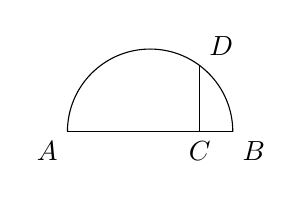
\begin{tikzpicture}[scale=2.1]
  \draw (0,0) -- (1,0);
  \draw (0,0) arc (180:0:0.5);
  \draw (0.8,0) -- (0.8,0.4);
  \node[below left] at (0,0) {$A$};
  \node[below right] at (1,0) {$B$};
  \node[below] at (0.8,0) {$C$};
  \node[above right] at (0.8,0.4) {$D$};
\end{tikzpicture}
\end{center}
\nopagebreak[4]
\Needspace{4\baselineskip}
\textbf{解析}

\Needspace{5\baselineskip}
半圆的直径为 $AB$，且 $CD\perp AB$，所以由直角三角形斜边上的高的性质，

\nopagebreak[4]
\[
CD^2=AC\cdot CB
\]

\Needspace{5\baselineskip}
由 $AB=1$、$AC:CB=4:1$，可得

\nopagebreak[4]
\[
AC=\frac45\qquad CB=\frac15
\]

\Needspace{5\baselineskip}
于是

\nopagebreak[4]
\[
CD=\sqrt{\frac45\cdot\frac15}
=\sqrt{\frac4{25}}
=\frac25
\]

\gkanswer{答案：$CD=\dfrac25$。}

\end{answer}
\begin{answer}
\gksolhead{4}{}

\textbf{题目}：

从二面角内任意一点向二面角的两个面作垂线，求证这两条垂线所决定的平面垂直于二面角的棱。（要求画图）

\Needspace{4\baselineskip}
\textbf{解析}

设二面角为 $M\text{-}AB\text{-}N$，点 $P$ 在二面角内；从 $P$ 分别向平面 $M$、平面 $N$ 作垂线，垂足为 $C$、$D$。原卷图形按如下 TikZ 矢量源重绘。
\nopagebreak[4]
\begin{center}\begin{tikzpicture}[scale=0.9,>=Stealth]
  % 两个面的示意投影与公共棱 AB
  \fill[gray!10] (0,0) -- (4,0) -- (5,1.1) -- (1,1.1) -- cycle;
  \fill[gray!18] (0,0) -- (1,1.1) -- (2.2,3.2) -- (1.2,2.1) -- cycle;
  \draw (0,0) -- (4,0) -- (5,1.1) -- (1,1.1) -- cycle;
  \draw (0,0) -- (1,1.1) -- (2.2,3.2) -- (1.2,2.1) -- cycle;
  \draw[very thick] (0,0) -- (1,1.1) node[midway,above left] {$AB$};
  \coordinate (P) at (2.1,1.7);
  \coordinate (C) at (1.25,1.1);
  \coordinate (D) at (2.1,2.55);
  \draw[thick] (P) -- (C) node[pos=0,anchor=north west,xshift=5pt,yshift=2pt] {$PC$};
  \draw[thick] (P) -- (D) node[midway,right] {$PD$};
  \fill (P) circle (1.4pt) node[above right] {$P$};
  \fill (C) circle (1.2pt) node[below right,yshift=-3pt] {$C$};
  \fill (D) circle (1.2pt) node[above right] {$D$};
  \node at (3.5,0.45) {$M$};
  \node at (1.55,2.85) {$N$};
\end{tikzpicture}
\end{center}
\nopagebreak[4]
因为 $PC\perp$ 平面 $M$，而 $AB$ 在平面 $M$ 内，所以 $PC\perp AB$。同理，$PD\perp AB$。

\Needspace{5\baselineskip}
直线 $PC$、$PD$ 是平面 $PCD$ 内相交的两条直线，并且都垂直于 $AB$，因此

\nopagebreak[4]
\[
\text{平面 }PCD\perp AB
\]

也可以从面面垂直的性质说明：过 $PC$ 的平面 $PCD$ 垂直于平面 $M$，过 $PD$ 的平面 $PCD$ 垂直于平面 $N$；而 $AB$ 是平面 $M$、$N$ 的交线，所以平面 $PCD$ 垂直于交线 $AB$。

\gkanswer{答案：见解析版。}

\end{answer}
\begin{answer}
\gksolhead{5}{}

\textbf{题目}：

\Needspace{5\baselineskip}
利用下列常用对数表，计算

\nopagebreak[4]
\[
23.28^{-1.1}
\]

常用对数表（原表右侧的数字为平均差栏；为适合 A4 黑白打印，整理为两张窄表，数据不变）：

\scriptsize

\begin{center}
\begingroup\setlength{\tabcolsep}{4pt}
\begin{tabular}{crrrrrrrrrr}
\toprule
$N$ & 0 & 1 & 2 & 3 & 4 & 5 & 6 & 7 & 8 & 9 \\
\midrule
23 & 3617 & 3636 & 3655 & 3674 & 3692 & 3711 & 3729 & 3747 & 3766 & 3784 \\
24 & 3802 & 3820 & 3838 & 3856 & 3874 & 3892 & 3909 & 3927 & 3945 & 3962 \\
25 & 3979 & 3997 & 4014 & 4031 & 4048 & 4065 & 4082 & 4099 & 4116 & 4133 \\
\bottomrule
\end{tabular}
\endgroup
\end{center}

\normalsize

常用对数表平均差栏：

\scriptsize

\begin{center}
\begingroup\setlength{\tabcolsep}{4pt}
\begin{tabular}{crrrrrrrrr}
\toprule
$N$ & 1 & 2 & 3 & 4 & 5 & 6 & 7 & 8 & 9 \\
\midrule
23 & 2 & 4 & 6 & 7 & 9 & 11 & 13 & 15 & 17 \\
24 & 2 & 4 & 5 & 7 & 9 & 11 & 12 & 14 & 16 \\
25 & 2 & 3 & 5 & 7 & 9 & 10 & 12 & 14 & 15 \\
\bottomrule
\end{tabular}
\endgroup
\end{center}

\normalsize

反对数表（同样将主体和平均差栏分开）：

\scriptsize

\begin{center}
\begingroup\setlength{\tabcolsep}{4pt}
\begin{tabular}{crrrrrrrrrr}
\toprule
$m$ & 0 & 1 & 2 & 3 & 4 & 5 & 6 & 7 & 8 & 9 \\
\midrule
.48 & 3020 & 3027 & 3034 & 3041 & 3048 & 3055 & 3062 & 3069 & 3076 & 3083 \\
.49 & 3090 & 3097 & 3105 & 3112 & 3119 & 3126 & 3133 & 3141 & 3148 & 3155 \\
.50 & 3162 & 3170 & 3177 & 3184 & 3192 & 3199 & 3206 & 3214 & 3221 & 3228 \\
\bottomrule
\end{tabular}
\endgroup
\end{center}

\normalsize

反对数表平均差栏：

\scriptsize

\begin{center}
\begingroup\setlength{\tabcolsep}{4pt}
\begin{tabular}{crrrrrrrrr}
\toprule
$m$ & 1 & 2 & 3 & 4 & 5 & 6 & 7 & 8 & 9 \\
\midrule
.48 & 1 & 1 & 2 & 3 & 4 & 4 & 5 & 6 & 6 \\
.49 & 1 & 1 & 2 & 3 & 4 & 4 & 5 & 6 & 6 \\
.50 & 1 & 1 & 2 & 3 & 4 & 4 & 5 & 6 & 7 \\
\bottomrule
\end{tabular}
\endgroup
\end{center}

\normalsize

\Needspace{4\baselineskip}
\textbf{解析}

\Needspace{5\baselineskip}
由常用对数表，$23.28$ 的常用对数为

\nopagebreak[4]
\[
\lg23.28=1.3670
\]

\Needspace{5\baselineskip}
因此

\nopagebreak[4]
\[
\lg(23.28^{-1.1})=-1.1\lg23.28
=-1.1\times1.3670=-1.5037
\]

\Needspace{5\baselineskip}
按常用对数中负特征数的写法，

\nopagebreak[4]
\[
-1.5037=\overline{2}.4963
\]

\Needspace{5\baselineskip}
查反对数表，得到

\nopagebreak[4]
\[
23.28^{-1.1}=0.03135
\]

\gkanswer{答案：$23.28^{-1.1}=0.03135$。}

\end{answer}
\gkpart{二、大题}

\begin{answer}
\gksolhead{6}{}

\textbf{题目}：

\Needspace{5\baselineskip}
解方程：

\nopagebreak[4]
\[
\sin3x-\sin x+\cos2x=0
\]

\Needspace{4\baselineskip}
\textbf{解析}

\Needspace{5\baselineskip}
由正弦的三倍角公式和差化积公式，

\nopagebreak[4]
\[
\sin3x-\sin x=2\cos2x\sin x
\]

\Needspace{5\baselineskip}
所以原方程等价于

\nopagebreak[4]
\[
\cos2x(2\sin x+1)=0
\]

\Needspace{5\baselineskip}
当 $\cos2x=0$ 时，

\nopagebreak[4]
\[
2x=\frac\pi2+n\pi
\qquad x=\frac\pi4+\frac{n\pi}{2}=n\pi\pm\frac\pi4
\]

\Needspace{5\baselineskip}
当 $2\sin x+1=0$ 时，$\sin x=-\dfrac12$，因此

\nopagebreak[4]
\[
x=2n\pi-\frac\pi6
\qquad x=(2n+1)\pi+\frac\pi6
\qquad n\in\mathbb Z
\]

\Needspace{5\baselineskip}
综上，

\nopagebreak[4]
\[
x=n\pi\pm\frac\pi4
\quad x=2n\pi-\frac\pi6
\quad x=(2n+1)\pi+\frac\pi6
\qquad n\in\mathbb Z
\]

\gkanswer{答案：$x=n\pi\pm\dfrac\pi4$，或 $x=2n\pi-\dfrac\pi6$，或 $x=(2n+1)\pi+\dfrac\pi6$，其中 $n\in\mathbb Z$。}

\end{answer}
\begin{answer}
\gksolhead{7}{}

\textbf{题目}：

用 $1,2,3,4,7,9$ 组成没有重复数字的五位数，问：

（1） 这样的五位数一共有多少个？

（2） 在这些五位数中，有多少个是偶数？

（3） 在这些五位数中，有多少个是 $3$ 的倍数？

\Needspace{4\baselineskip}
\textbf{解析}

\gksubpart{（1）}

\Needspace{5\baselineskip}
从 $1,2,3,4,7,9$ 中取出 $5$ 个并排列，得到

\nopagebreak[4]
\[
A_6^5=6\times5\times4\times3\times2=720
\]

\gksubpart{（2）}

\Needspace{5\baselineskip}
五位偶数的末位只能取 $2$ 或 $4$，有 $2$ 种选择；确定末位后，从剩下的 $5$ 个数字中取 $4$ 个排列，故共有

\nopagebreak[4]
\[
2A_5^4=2\times(5\times4\times3\times2)=240
\]

个偶数。

\gksubpart{（3）}

\Needspace{5\baselineskip}
六个数字的和为

\nopagebreak[4]
\[
1+2+3+4+7+9=26
\]

\Needspace{5\baselineskip}
五位数是 $3$ 的倍数，当且仅当所用五个数字的和是 $3$ 的倍数。只有去掉 $2$ 后，剩余数字 $1,3,4,7,9$ 的和为 $24$，所以这五个数字必须全部使用，排列数为

\nopagebreak[4]
\[
P_5=5!=120
\]

\gkanswer{答案（1）：$720$ 个。}

\gkanswer{答案（2）：$240$ 个。}

\gkanswer{答案（3）：$120$ 个。}

\end{answer}
\begin{answer}
\gksolhead{8}{}

\textbf{题目}：

\Needspace{5\baselineskip}
解方程组：

\nopagebreak[4]
\[
\begin{cases}
x^2-2xy-y^2=1,\\[2pt]
\sqrt{xy+3}=x.
\end{cases}
\]

（限定在实数范围内。）

\Needspace{4\baselineskip}
\textbf{解析}

\Needspace{5\baselineskip}
原方程组的第二式为根式方程，平方时必须把候选解代回原式检查。由

\nopagebreak[4]
\[
\sqrt{xy+3}=x
\]

\Needspace{5\baselineskip}
可知 $x\geq0$，平方得

\nopagebreak[4]
\[
xy+3=x^2
\qquad x^2-xy=3
\]

\Needspace{5\baselineskip}
将第一式乘以 $3$，再减去上式，得到

\nopagebreak[4]
\[
2x^2-5xy-3y^2=0
= (2x+y)(x-3y)
\]

因此分两种情况。

当 $2x+y=0$ 时，$y=-2x$。代入 $x^2-xy=3$，得 $3x^2=3$，所以 $x=\pm1$。由 $x\geq0$ 及原根式方程，保留 $(x,y)=(1,-2)$。

\Needspace{5\baselineskip}
当 $x-3y=0$ 时，$x=3y$。代入 $x^2-xy=3$，得 $6y^2=3$，于是 $y=\pm\dfrac{\sqrt2}{2}$，$x=\pm\dfrac{3\sqrt2}{2}$。由 $x\geq0$ 并代回原方程，保留

\nopagebreak[4]
\[
\left(x,y\right)=\left(\frac{3\sqrt2}{2},\frac{\sqrt2}{2}\right)
\]

\Needspace{5\baselineskip}
故方程组的解为

\nopagebreak[4]
\[
(x,y)=(1,-2)\qquad
\left(x,y\right)=\left(\frac{3\sqrt2}{2},\frac{\sqrt2}{2}\right)
\]

\gkanswer{答案：$(x,y)=(1,-2)$ 或 $\left(\dfrac{3\sqrt2}{2},\dfrac{\sqrt2}{2}\right)$。}

\end{answer}
\begin{answer}
\gksolhead{9}{}

\textbf{题目}：

\Needspace{5\baselineskip}
如图，线段 $CD$ 与 $\odot O$ 相交于 $A\text{、}B$ 两点，且 $AC=BD$，又 $CE\text{、}DF$ 分别与 $\odot O$ 相切于 $E\text{、}F$。求证：

\nopagebreak[4]
\[
\triangle OEC\cong\triangle OFD
\]
\nopagebreak[4]
\begin{center}\begin{tikzpicture}[scale=1.45,>=Stealth]
  \coordinate (O) at (0,0);
  \coordinate (C) at (-1.7,0);
  \coordinate (A) at (-0.72,0);
  \coordinate (B) at (0.72,0);
  \coordinate (D) at (1.7,0);
  \coordinate (E) at (-0.588,0.809);
  \coordinate (F) at (0.588,-0.809);
  \draw (O) circle (1);
  \draw[thick] (C) -- (D);
  \draw[thick] (C) -- (E);
  \draw[thick] (D) -- (F);
  \draw[dashed] (O) -- (E) (O) -- (F);
  \fill (O) circle (1.2pt) node[below] {$O$};
  \fill (A) circle (1.2pt) node[above] {$A$};
  \fill (B) circle (1.2pt) node[above] {$B$};
  \fill (C) circle (1.2pt) node[below left] {$C$};
  \fill (D) circle (1.2pt) node[below right] {$D$};
  \fill (E) circle (1.2pt) node[above left] {$E$};
  \fill (F) circle (1.2pt) node[below right] {$F$};
\end{tikzpicture}
\end{center}
\nopagebreak[4]
\Needspace{4\baselineskip}
\textbf{解析}

\Needspace{5\baselineskip}
连接 $OA\text{、}OB$。因为 $OA=OB$，所以在等腰三角形 $OAB$ 中

\nopagebreak[4]
\[
\angle OAB=\angle OBA
\]

\Needspace{5\baselineskip}
又因 $C,A,B,D$ 共线，得到

\nopagebreak[4]
\[
\angle OAC=\angle OBD
\]

\Needspace{5\baselineskip}
结合 $AC=BD$ 和 $OA=OB$，可得

\nopagebreak[4]
\[
\triangle OAC\cong\triangle OBD
\qquad OC=OD
\]

\Needspace{5\baselineskip}
切线分别在 $E\text{、}F$ 处与圆相切，所以

\nopagebreak[4]
\[
OE\perp CE\qquad OF\perp DF\qquad OE=OF
\]

\Needspace{5\baselineskip}
于是直角三角形 $OEC$ 与 $OFD$ 的斜边 $OC\text{、}OD$ 相等，且一条直角边 $OE\text{、}OF$ 相等，故由斜边直角边判定

\nopagebreak[4]
\[
\triangle OEC\cong\triangle OFD
\]

\gkanswer{答案：见解析版。}

\end{answer}
\begin{answer}
\gksolhead{10}{}

\textbf{题目}：

如图，半径为 $1$ 的球内切于圆锥（即直圆锥），已知圆锥的母线与底面的夹角是 $2\theta$。

\Needspace{5\baselineskip}
（1） 求证圆锥的母线与底面半径的和是

\nopagebreak[4]
\[
\frac{2}{\tan\theta\left(1-\tan^2\theta\right)}
\]

\Needspace{5\baselineskip}
（2） 求证圆锥的全面积是

\nopagebreak[4]
\[
\frac{2\pi}{\tan^2\theta\left(1-\tan^2\theta\right)}
\]

（3） 当 $\theta$ 是什么值的时候，圆锥的全面积最小？（$\theta$ 用反三角函数表示。）

图中 $V$ 是圆锥的顶点，$VB$ 是母线，$O$ 是球心，$A$ 是球和圆锥底面的切点。
\nopagebreak[4]
\begin{center}\begin{tikzpicture}[scale=0.82,>=Stealth]
  \coordinate (V) at (0,4.5);
  \coordinate (B) at (-1.35,0);
  \coordinate (A) at (0,0);
  \coordinate (O) at (0,1);
  \coordinate (C) at (-0.49,1.64);
  \draw[thick] (V) -- (B) -- (A) -- cycle;
  \draw[dashed] (V) -- (A);
  \draw (O) circle (1);
  \draw[dashed] (-1.35,0) arc (180:360:1.35 and 0.28);
  \draw (B) arc (180:360:1.35 and 0.28);
  \draw[thick] (O) -- (A);
  \draw[thick] (O) -- (C);
  \draw pic[draw,angle radius=0.35cm,"$2\theta$" {shift={(0.08,0.12)}}]
    {angle=A--B--V};
  \fill (V) circle (1.3pt) node[above] {$V$};
  \fill (B) circle (1.3pt) node[below left] {$B$};
  \fill (A) circle (1.3pt) node[below right] {$A$};
  \fill (O) circle (1.3pt) node[right] {$O$};
  \fill (C) circle (1.3pt) node[left] {$C$};
\end{tikzpicture}
\end{center}
\nopagebreak[4]
\Needspace{4\baselineskip}
\textbf{解析}

\gksubpart{（1）}

\Needspace{5\baselineskip}
在圆锥的轴截面内，设 $C$ 为母线 $VB$ 与球的切点。连接 $OA\text{、}OB\text{、}OC$。由于球半径为 $1$，有

\nopagebreak[4]
\[
OA=OC=1\qquad \angle OAB=\angle OCB=90^\circ\qquad OB=OB
\]

\Needspace{5\baselineskip}
所以直角三角形 $OAB$ 与 $OCB$ 全等，从而

\nopagebreak[4]
\[
\angle OBA=\angle OBC=\theta
\]

\Needspace{5\baselineskip}
设圆锥底面半径为 $r$，母线长为 $l$。在直角三角形 $OAB$ 中，

\nopagebreak[4]
\[
\tan\theta=\frac{OA}{AB}=\frac1r
\qquad r=\cot\theta
\]

\Needspace{5\baselineskip}
母线 $VB$ 与底面的夹角为 $2\theta$，故其在底面半径方向的投影给出

\nopagebreak[4]
\[
r=l\cos2\theta
\qquad l=\frac{r}{\cos2\theta}
\]

\Needspace{5\baselineskip}
于是

\nopagebreak[4]
\[
\begin{gathered}
l+r=\cot\theta\left(\frac1{\cos2\theta}+1\right)\\
=\frac1{\tan\theta}\cdot\frac{1+\cos2\theta}{\cos2\theta}\\
=\frac1{\tan\theta}\cdot\frac{2\cos^2\theta}{\cos2\theta}\\
=\frac{2}{\tan\theta\left(1-\tan^2\theta\right)}
\end{gathered}
\]

\gksubpart{（2）}

\Needspace{5\baselineskip}
圆锥的全面积为

\nopagebreak[4]
\[
T=\pi rl+\pi r^2=\pi r(l+r)
\]

\Needspace{5\baselineskip}
代入 $r=\cot\theta$ 以及上式，得

\nopagebreak[4]
\[
T=\frac{2\pi}{\tan^2\theta\left(1-\tan^2\theta\right)}
\]

\gksubpart{（3）}

\Needspace{5\baselineskip}
在圆锥的几何范围内令 $u=\tan^2\theta$，则 $0<u<1$，且

\nopagebreak[4]
\[
u(1-u)=-\left(u-\frac12\right)^2+\frac14
\]

\Needspace{5\baselineskip}
因此 $u(1-u)$ 在 $u=\dfrac12$ 时取得最大值，全面积 $T$ 取得最小值。故

\nopagebreak[4]
\[
\tan^2\theta=\frac12
\qquad \theta=\arctan\frac{\sqrt2}{2}
\]

\gkanswer{答案（1）：$l+r=\dfrac{2}{\tan\theta(1-\tan^2\theta)}$。}

\gkanswer{答案（2）：$T=\dfrac{2\pi}{\tan^2\theta(1-\tan^2\theta)}$。}

\gkanswer{答案（3）：$\theta=\arctan\dfrac{\sqrt2}{2}$ 时全面积最小。}

\end{answer}